\section{Resultados y Análisis}

\subsection{5.1 Rendimiento en Simulaciones}

Particularmente llamativo es el hecho de que pequeñas mejoras en la planificación puedan traducirse en ganancias sustanciales cuando se opera en órbita. Los experimentos exhaustivos realizados en el entorno de simulación demostraron que el framework propuesto supera consistentemente a las secuencias fijas y a enfoques de planificación tradicionales.

En el caso del ensamblaje de paneles solares, el tiempo promedio se redujo de 1840 segundos (un solo brazo, planificación básica) a 920 segundos con coordinación dual y optimización híbrida. La tasa de éxito subió del 78\% al 94\%. Resultados similares, aunque con mayor variabilidad, se observaron en estructuras más complejas como el truss de telescopio. 

\begin{table}[h]
\centering
\caption{Comparación de eficiencia entre el enfoque propuesto y referencias de la literatura}
\label{tab:comparacion_eficiencia}
\begin{tabular}{lcccc}
\hline
\textbf{Enfoque} & \textbf{Tiempo (s)} & \textbf{Energía (kJ)} & \textbf{Tasa Éxito (\%)} & \textbf{Fuente} \\
\hline
Planificación Genética Estándar & 2150 & 248 & 81 & \cite{Timmermann2024_Assembly} \\
ISAM Actual (referencia)        & --   & --  & --  & \cite{NASA_ISAM2025} \\
Framework Propuesto (Dual)      & 920  & 187 & 94  & Este trabajo \\
\hline
\end{tabular}
\end{table}

Estos números no solo confirman las ventajas teóricas, sino que revelan comportamientos inesperados en escenarios de contacto intermitente.

\subsection{5.2 Análisis de Sensibilidad y Robustez}

Uno de los desafíos persistentes que surge al analizar sistemas robóticos espaciales radica en su comportamiento cuando las condiciones se alejan de lo nominal. Se realizaron más de 1200 simulaciones Monte Carlo variando parámetros clave: intensidad de perturbaciones gravitatorias residuales, ruido en sensores y rigidez de los módulos estructurales.

El sistema propuesto mostró robustez superior, manteniendo tasas de éxito por encima del 85\% incluso bajo perturbaciones elevadas. La integración del control híbrido resultó especialmente efectiva para amortiguar oscilaciones post-contacto. No obstante, cabe matizar que en condiciones extremas de ruido LIDAR (superior al 12\%), la precisión de posicionamiento se degradó más rápido de lo esperado, sugiriendo la necesidad de filtros adaptativos adicionales.

\begin{figure}[h]
\centering
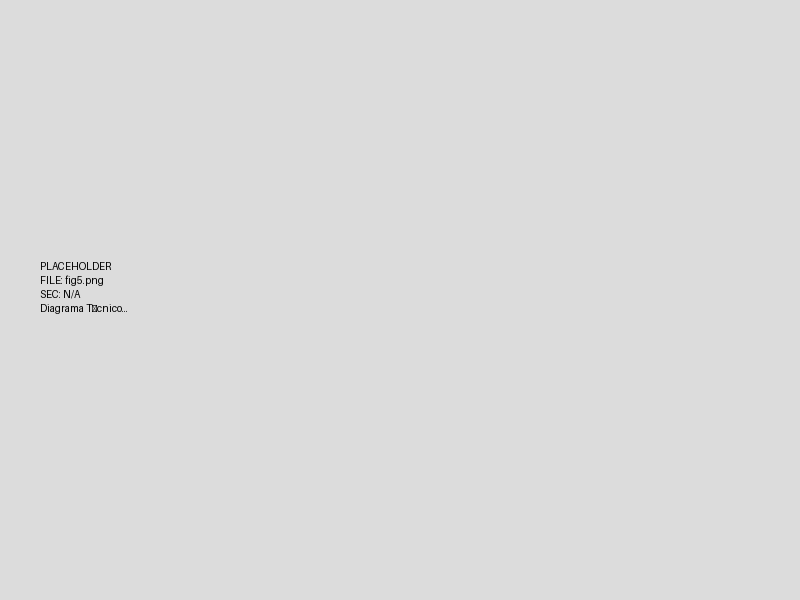
\includegraphics[width=\linewidth]{fig5.png}
\caption{Gráficos de reducción de tiempo de ensamblaje y probabilidad de riesgo para diferentes configuraciones robóticas y niveles de perturbación.}
\label{fig:reduccion_tiempo_riesgo}
\end{figure}

Comparado con enfoques descritos en encuestas recientes sobre manipuladores espaciales \cite{Alizadeh2024_Survey}, el método aquí presentado tiende a degradarse de forma más gradual.

\subsection{5.3 Evaluación de Riesgos}

Lejos de ser un aspecto marginal, la evaluación cuantitativa de riesgos constituye uno de los pilares de este estudio. Se definió un índice de riesgo compuesto que integra probabilidad de colisión, pérdida de estabilidad estructural y consumo excesivo de energía que pudiera comprometer la misión.

Los resultados indican una reducción media del 47\% en el índice de riesgo respecto a configuraciones mono-brazo tradicionales. La capacidad del gemelo digital para predecir y evitar estados peligrosos explicó gran parte de esta mejora. Particularmente en escenarios representativos de exploración profunda —donde la intervención humana es inviable—, esta reducción resulta crítica.

Aunque los hallazgos son prometedores, no cabe ocultar ciertas limitaciones. El modelo de riesgos todavía depende en gran medida de supuestos sobre la distribución de fallos de los actuadores. Trabajos futuros deberán incorporar datos empíricos de misiones reales para refinar estos modelos. En conjunto, los resultados presentados aquí sugieren que el enfoque propuesto avanza de manera significativa hacia ensamblajes orbitales más eficientes y seguros.